\chapter{Lecture 3 - The Bisection Method}
\label{ch:lec3n}
\section{Objectives}
The objectives of this lecture are to:
\begin{itemize}
\item Introduce the problem of solving non-linear equations.
\item Describe the bisection method.
\item Discuss error estimates and stopping criteria.
\item Illustrate the bisection method with an example.
\end{itemize}
\setcounter{lstannotation}{0}

\section{Solving Non-Linear Equations}
Engineers often need to solve non-linear equations.  An equation of one variable can be written in the form:
\begin{equation}
f(x) = 0
\end{equation}
A solution to such an equation is called a \emph{root}.  In past lectures, in the analytical methods portion of this text, we frequently needed to find the root(s) of linear and non-linear equations.  We also encountered several cases where we were not able to find the roots analytically.\sidenote{As a quick re-cap: 
\begin{itemize}
\item In lecture 19 we needed to find the roots of $J_{0}(x)$.  We did not write our own routine for doing this but, at its heart, \lstinline[style=myMatlab]{besselzero()} had to solve a non-linear equation.  We used these tools again in lectures 31, 32, and 33 along with several homework problems.
\item In lecture 28 we needed to find roots of $f(x) = \tan{x} + \sfrac{x}{h}$ for a given value of $h$.
\end{itemize}
}
The case that this lecture will address is when such roots cannot be found analytically.  As an example, suppose we wish to find the area marked $A_s$ as shown in Figure \ref{fig:lec3n-ex1} which is given in Equation \ref{eq:lec3n-ex1}.
\begin{marginfigure}
\includegraphics{Chapter3_fig3_2.jpg}
\caption{Schematic of example.}
\label{fig:lec3n-ex1}
\end{marginfigure}
\begin{equation}
A_s = \frac{1}{2}r^2\left(\theta - \sin{\theta}\right)
\label{eq:lec3n-ex1}
\end{equation}
where $A_s$ and $r$ are given.  This is a non-linear equation and we wish to solve it numerically.

\newthought{There are two} general approaches with numerical methods to solve non-linear equations:
\begin{enumerate}
\item bracketing methods; and
\item open methods.
\end{enumerate}
In bracketing methods, we start with an interval in which we know a root to lie.  Each step of the algorithm seeks to reduce the size of the interval while always maintaining the root inside.  When the interval is small enough, we have effectively found the root.  In open methods no such bounding interval is maintained.  We start with an estimate of the root and, through successive iterations of the algorithm, attempt to improve our estimate.  The iteration stops when our estimation of the root meets a specified termination criterion.  

\section{Bisection Method}
The bisection method is a bracketing method for finding a root of a \emph{continuous} function when it is known that the root lies within a specified interval: $x \in [a,b]$.  The bisection method consists of the following steps:

\begin{marginfigure}
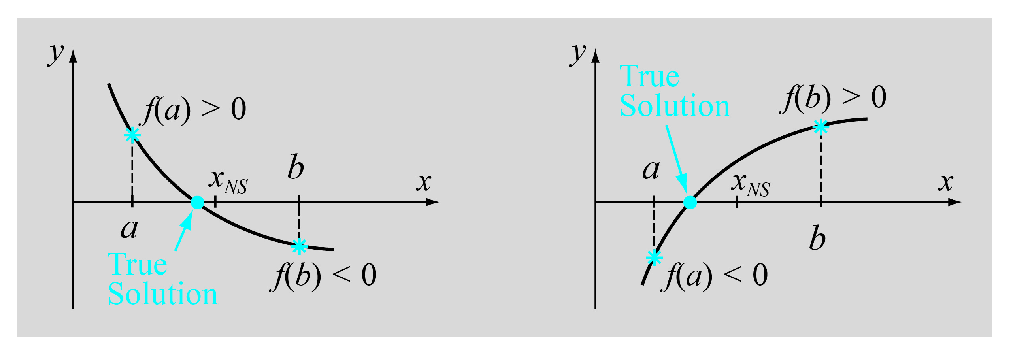
\includegraphics{Chapter3_Fig3_6.eps}
\caption{Solution of $f(X)=0$ must lie in $[a,b]$ if $f(a)f(b)<0$.}
\label{fig:lec3n-bisection-schematic}
\end{marginfigure}
\begin{enumerate}
\item Find an interval $[a,b]$ in which a root exists.  One way to find such an interval is to identify an $a$ and $b$ for which $f(a)f(b)<0$.  As is illustrated in Figure \ref{fig:lec3n-bisection-schematic}, if $f(x)$ is continuous, this is a sufficient condition for a root to exist in $[a,b]$.\sidenote{\textbf{Note:} How one goes about determining a suitable $a$ and $b$ is not part of the algorithm.}

\item Calculate an estimate of the numerical solution from Equation \ref{eq:lec3n-bisection-est}:
\begin{equation}
x_{\text{NS}} = \frac{(a+b)}{2}
\label{eq:lec3n-bisection-est}
\end{equation}

\item Determine whether the root is in $[a,x_{\text{NS}}]$ or in $[x_{\text{NS}},b]$ using the following method:
\begin{itemize}
\item If $f(a)f(x_{\text{NS}}) < 0$, the root is in $[a,x_{\text{NS}}]$.
\item If $f(x_{\text{NS}})f(b) < 0$, the root is in $[x_{\text{NS}},b]$.
\end{itemize}
Except in the edge case that $f(x_{\text{NS}})=0$, only one of the above conditions will be true.\sidenote[][-1.5cm]{\textbf{Health Warning:} You should definitely test this edge case.}

\item Select the subinterval that contains the solution---either $[a,x_{\text{NS}},b]$ or $[x_{\text{NS}},b]$ as determined in step 3---as the new $a$ and $b$ and return to step 2.
\end{enumerate}
Three iterations of the bisection method are illustrated in Figure \ref{fig:lec3n-bisection-first-three}.
\begin{marginfigure}
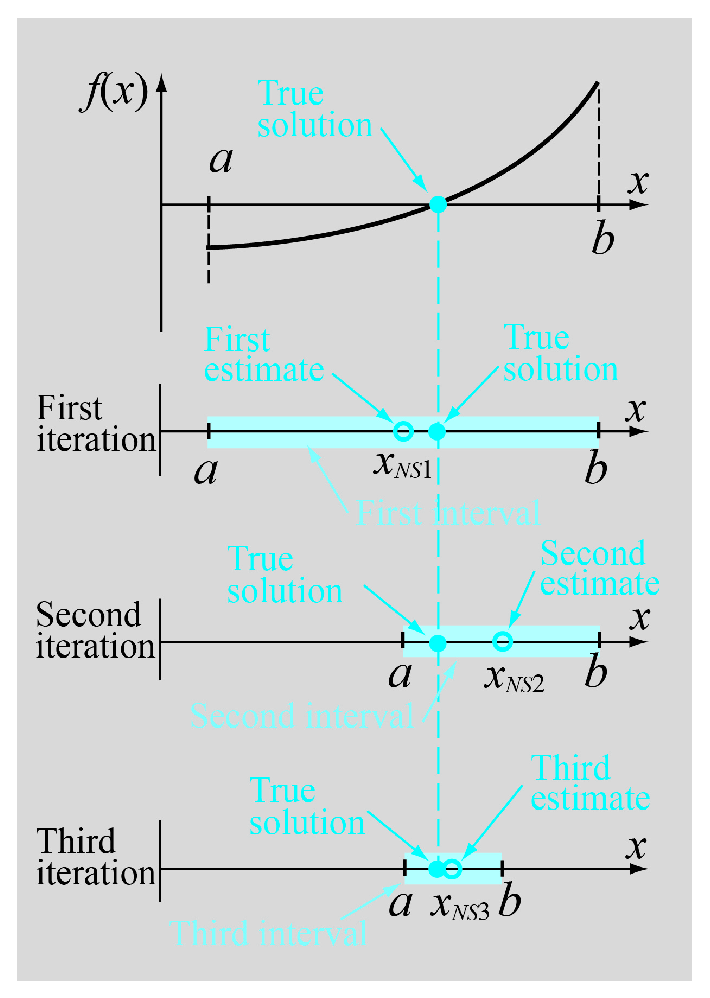
\includegraphics{Chapter3_Fig3_7.eps}
\caption{First three iterations of the bisection method.}
\label{fig:lec3n-bisection-first-three}
\end{marginfigure}

\newthought{Here we offer} some comments on the bisection method.

\begin{enumerate}
\item If $f(x)$ is continuous and exactly one root is contained in the initial interval $[a,b]$, the bisection method is guaranteed to converge with the error in $x_{\text{NS}}$ reduced by a factor of two with each iteration of the algorithm.
\item The convergence rate is steady but slow relative to other methods.\sidenote{Since the error is reduced by a constant fraction with each iteration, the bisection method is said to exhibit \emph{linear convergence}.}
\item The test $f(a)f(b)<0$ is a \emph{sufficient} condition for a root to exist between $[a,b]$ but is not a \emph{necessary} condition.  For example, the function $f(x)=\left(x-3\right)^2$ has two roots at $x=3$, but with $a=1$ and $b=4$, we find that $f(1)f(4)>0$ and the test fails.
\item The algorithm is tailored to find just one root.  If multiple roots are desired, one must change the algorithm accordingly.
\end{enumerate}
We will do an example problem, but before we get to that, a quick discussion of error estimation is in order.

\section{Error Estimates and Stopping Criteria}
Error estimation plays an essential role in bracketing algorithms.  After all:
\begin{enumerate}
\item Such algorithms do not really ``find'' the root; instead the algorithm starts with an interval in which the root lies and steps of the algorithm are carried out to make the interval arbitrarily small, all while keeping the root within the interval.  In this sense, while the precise real number that is the root of the equation is not found, we place the root within a range that is as small as is desired.

\item Indeed, if $f(x)$ is a non-linear equation, and $f(x^{\star})=0$,\marginnote{\textbf{Note:} We use the notation $x^{\star}$ to denote the \emph{exact solution}. In places we will also use the notation: $x_{\text{TS}}$ to denote the exact or \emph{true} solution.} there is no reason to expect that $x^{\star}$ can be exactly represented on the computer using double-precision floating point numbers.
\end{enumerate}
Consequently, no matter what result is produced from a bracketing method, we know it is in error.  Our job is to be mindful of this error and be sure that it is kept to within acceptable bounds.  In addition to controlling the magnitude of the error, bracketing algorithms customarily use error estimates as stopping criteria.  We stop the algorithm when the estimated error is reduced below a pre-defined threshold.

\vspace{0.25cm}

\noindent There are several standard error estimates that we will consider.

\begin{enumerate}
\item True error.  This is given by Equation \ref{eq:lec3n-true-error}.
\begin{equation}
\text{True error} = x^{\star} - x_{\text{NS}}
\label{eq:lec3n-true-error}
\end{equation}
This is not often used as a stopping criterion since, except in special testing cases, we generally do not know what the true solution, $x^{\star}$, is.

\vspace{3.0cm}

\item Tolerance in $f(x)$ given by Equation \ref{eq:lec3n-tol-in-f}.
\begin{equation}
\text{TOL} = \left| f(x^{\star}) - f(x_{\text{NS}}\right| = \left|0-\epsilon \right| = \left|\epsilon\right|
\label{eq:lec3n-tol-in-f}
\end{equation}
where $\epsilon$ is an error tolerance chosen by the user, e.g. $10^-6$.  The value of $f(x_{\text{NS}})$ is sometimes referred to as the \emph{residual}.  Use of this stopping criterion is generally only satisfactory if $f^{\prime}(x) \approx 1$ in the vicinity of the root.

\item Tolerance in the solution. If $x_{\text{NS}} = \sfrac{a+b}{2}$, then:
\begin{equation*}
\text{TOL} = \left|\frac{b-a}{2} \right|
\end{equation*}
which is half the subinterval.  This is a reasonable stopping criterion for the bisection method or any other bracketing method.\sidenote{Obviously, it is not suitable for non-bracketing algorithms since $a$ and $b$ would then be unknown.}  

\item Relative error.  For most numerical algorithms, if not necessarily the bisection method, the \emph{estimated relative error} is usually a good technique and is shown in Equation \ref{eq:lec3n-ere}.
\begin{equation}
\text{Estimated Relative Error} = \frac{\left|x_{\text{NS}}^{(n)} - x_{\text{NS}}^{(n-1)}\right|}{\left|x_{\text{NS}}^{(n-1)}\right|} 
\label{eq:lec3n-ere}
\end{equation}
where $x_{\text{NS}}^{(n)}$ is the estimated numeric solution at iteration $n$, and $x_{\text{NS}}^{(n-1)}$ is the estimated numeric solution at iteration $n-1$.  This error estimate has the advantage that it is a \emph{relative error measure} and takes into account the magnitude of $x_{\text{NS}}$.  A technical disadvantage arises if $x_{\text{NS}}$ is close to zero at any iteration.  
\end{enumerate}
Refinements on these stopping criteria will be discussed, as appropriate, throughout the course.

\section{MATLAB Implementation}

\textbf{Example:} You are tasked to estimate the pressure drop in a 0.1-m long section of a tube ($D=4.0$ mm diameter) that is used to transfer air with an average velocity of 50 m/s.  Under these conditions, the Reynolds number (Re)\marginnote[-1.5cm]{\textbf{Note:} Reynolds number is a non-dimensional parameter that relates the relative magnitude of inertial and viscous forces.  It is used to predict fluid flow patters.  The value of the Reynolds number is given by the equation:
$$\text{Re} = \frac{\rho \bar{v} \text{D}_c}{\mu}$$ where $\rho$ is fluid density, $\bar{v}$ is a characteristic---e.g. average---velocity, $\text{D}_c$ is some characteristic length, such as in this case the diameter of the tube, and $\mu$ is the fluid viscosity.  Higher Reynolds numbers (such as is given in this example) correspond to turbulent flow fields, low Reynolds number correspond to laminar flow.} of the air in the tube is approximately 13,700.  Assume the drawn tubing has an equivalent roughness $(\epsilon)$ of $0.0015$ mm.  As the first step, you plan to use the Colebrook equation to estimate the friction factor.  The Colebrook equation is given by:
\begin{equation*}
\frac{1}{\sqrt{f}} = -2.0 \log_{10}\left(\frac{\sfrac{\epsilon}{D}}{3.7} + \frac{2.51}{\text{Re}\sqrt{f}} \right)
\end{equation*}

We will start by clearing out the MATLAB workspace and encoding given data.
\begin{lstlisting}[name=lec3n-ex,style=myMatlab]
clear
clc
close 'all'

e = 0.0015; % mm, equialent roughness
D = 4.0; % mm, tube diameter
Re = 13700; % Reynolds number
\end{lstlisting}
Next we encode the nonlinear function whose roots we seek and select an initial interval in which we expect the root to reside.

\marginnote{
\ref{lst:ann3n-1} For the bisection method, these two stopping criteria may conflict.  We will use the tolerance in the solution criteria which, per the bisection algorithm, is halved with every iteration.  At the same time we are limiting the maximum number of iterations.  If the maximum number of iterations is too small, depending on the initial choice of $a$ and $b$, it may be impossible to satisfy the tolerance. The smallest tolerance you can satisfy is: $\text{TOL}_{\text{min}} = \left|\frac{b-a}{2^{\text{imax}}} \right|$ With the given choices of $a$, $b$, and \lstinline[style=myMatlab]{tol}, we should never reach the maximum specified number of iterations.  Still, it is okay to be conservative to guard against bugs.


\vspace{0.25cm}

\ref{lst:ann3n-2} Alternatively you might try to implement some routine that may automatically find an interval that spans a root.

}
\begin{lstlisting}[name=lec3n-ex, style=myMatlab]
F = @(f) 1./sqrt(f) + 2.0*log10((e/D)/3.7 + 2.51/(Re*sqrt(f)));

a = 0.001; b = 1; % initial interval
imax = 20; tol = 0.0001; % stopping criteria  /*!\annotation{lst:ann3n-1}!*/

Fa = F(a); Fb = F(b); 

% verify that Fa*Fb > 0
if (Fa*Fb > 0)
   error('Error: The function has the same sign at a and b'); /*!\annotation{lst:ann3n-2}!*/
end
\end{lstlisting}

Now we are ready to commence the bisection method.  In this listing we provide code necessary to provide outputs to the command window to update the user on the progress of the algorithm.
\marginnote{

\ref{lst:ann3n-3}  This is step \#2 of the bisection method.


\vspace{1.75 cm}  

\ref{lst:ann3n-4} Check the edge case where the root was exactly at the midpoint of the interval.

\vspace{0.25cm}

\ref{lst:ann3n-5} If the tolerance in the solution at iteration $i$ meets the stopping criterion, stop the iteration. The keyword \lstinline[style=myMatlab]{break} results in an immediate exit from the \lstinline[style=myMatlab]{for...end} loop.

\vspace{0.25cm}

\ref{lst:ann3n-6} Here we warn the user that the algorithm is about to be stopped based on maximum iterations.  Since the specified tolerance in the solution was never met, the user might want to re-start with a new (smaller) bracket, increase the tolerance, or increase the maximum allowed number of iterations.

\vspace{0.25cm}

\ref{lst:ann3n-7} This is step \#3 and step \#4 of the bisection method.

}
\begin{lstlisting}[name=lec3n-ex, style=myMatlab]
fprintf('iter       a         b            xNS         f(xNS)         Tol\n');
for i = 1:imax
   xNS = (a + b)/2; /*!\annotation{lst:ann3n-3}!*/
   toli = (b - a)/2;
   FxNS = F(xNS);
   fprintf('%3i %11.6f %11.6f  %11.6f  %11.6f  %11.6f\n',...
       i,a,b,xNS,FxNS,toli);
  
   if FxNS == 0
       fprintf('Exact solution x = %11.6f was found\n',xNS); /*!\annotation{lst:ann3n-4}!*/
       break;
   end   
   if toli < tol
       fprintf('Success!! x = %11.6f \n',xNS); /*!\annotation{lst:ann3n-5}!*/
       break; % end the loop since I meet my error tolerance
   end   
   % if toli > tol and i == imax, stop iteration.
   if i == imax                                        /*!\annotation{lst:ann3n-6}!*/
       fprintf('Solution not obtained in %i iterations\n',imax); 
       break
   end   
   % update bracket
   if (F(a)*FxNS < 0)
       b = xNS;
   else                   /*!\annotation{lst:ann3n-7}!*/
       a = xNS;
   end    
end

\end{lstlisting}
For this example problem the iteration succeeds and finds an estimated root at $x = 0.029109$ after 14 iterations.

\section{Summary}
The bisection method discussed in this lecture is useful.  It is both simple to implement in code and reliably converges to a root provided that a suitable initial interval is established.  The convergence rate is slow compared to the methods that we will explore in the next lecture. This slow convergence is not a significant problem for the problem types you are likely to encounter in a typical classroom environment; computers are fast and they do not mind working a little bit longer.  The convergence rate becomes an issue when evaluation of the function (to which we are finding a root) is computationally expensive.  Still, the bisection method is sufficient for most purposes.  In upcoming lectures we will explore improved algorithms.  One bracketing method we will discuss is called the regular falsi method.  It is introduced primarily as a way to show how one can try to make a good algorithm, like bisection method, better.
